Figure~\ref{fig:Drafting} shows the draft schedule establish for the first 8 weeks\emph{a priori}

\begin{figure*}
% - Use the starred version in order to put floats on two columns
% - Possibly, use the "\ifscreen ... \else ... \fi"" alternative to orientate correctly
%   the planning with respect to the orientation of the paper (cf. below for the auto-evaluation)
   \centering
      
  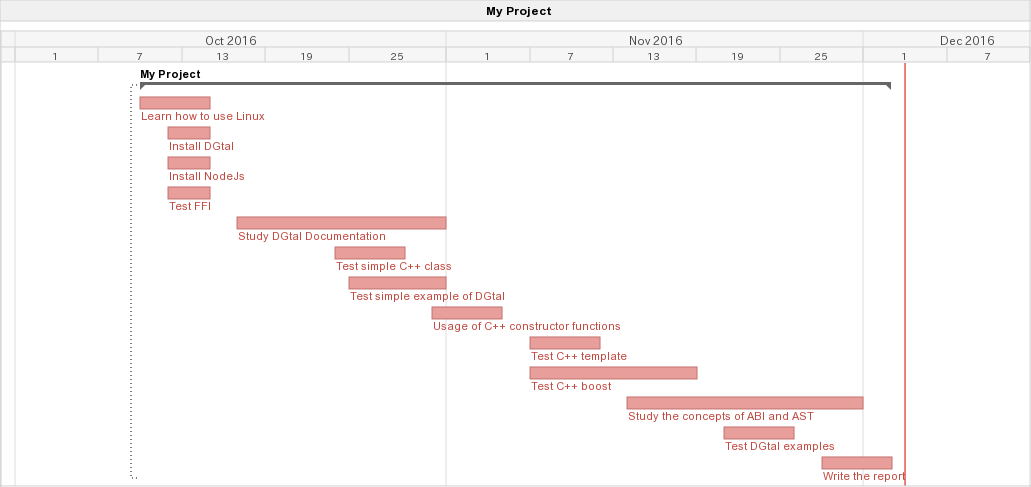
\includegraphics[scale=0.5]{Images/Gantt1.png}
  
   \caption{Drafting}
   \label{fig:Drafting}
\end{figure*}

Figure~\ref{fig:Planning} introduce the planning that has been build week after week during the course of the work for the first 8 weeks.

\begin{figure*}
   \centering
      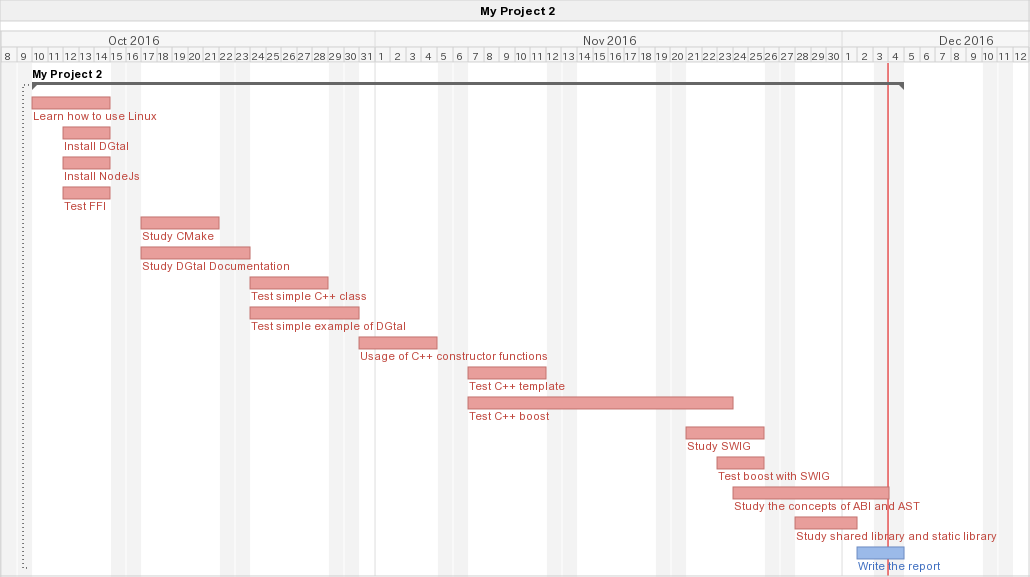
\includegraphics[scale=0.5]{Images/Gantt2.png}
      \caption{Planning}
   \label{fig:Planning}
\end{figure*}

There are two main difference of the drafting and the planning for the first 8 weeks. We have planned to study the documentation and test the examples of DGtal at very first time. However, the truth is we have under estimated of complexity of DGtal. The second difference is I've found the latest versions of SWIG can wrap c++ code for JavaScript, so I've spent quiet a lot of time to study it. 


Figure~\ref{fig:Drafting2} shows the draft schedule establish for week 9 to week 18\emph{a priori}


Figure~\ref{fig:Planning2} introduce the actual planning for week 9 to week 18.

The main difference of drafting and planning in this phase is in last week of January. As described in the weekly report, I was struggling to find an internship this week, because I failed all interviews that I had participated and I was so nervous this week. 
Luckily, I got an ideal offer at the beginning of February. But the works for this project is delayed to the next week.


\begin{figure*}
   \centering
      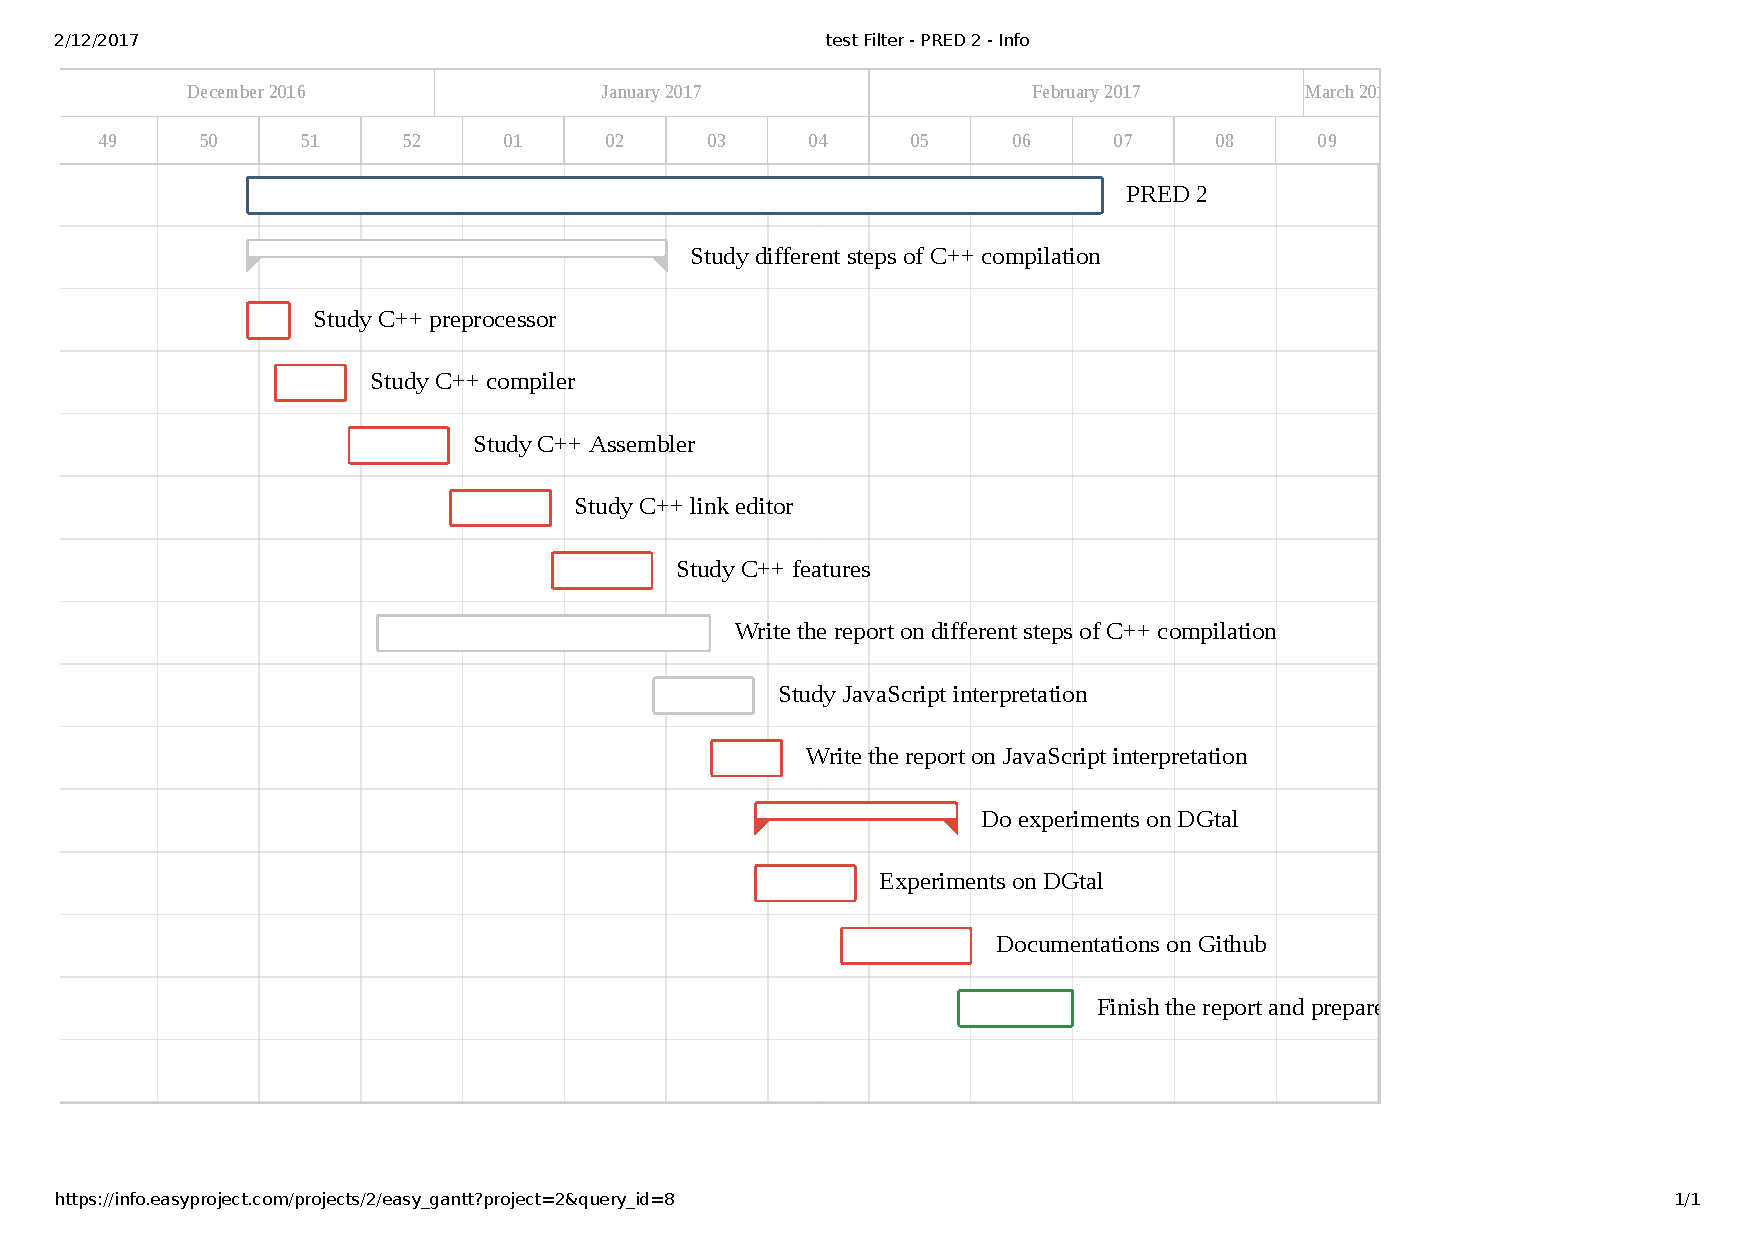
\includegraphics[scale=0.6]{Images/Gantt3.pdf}
      \caption{Drafting 2}
   \label{fig:Drafting2}
\end{figure*}


\begin{figure*}
   \centering
      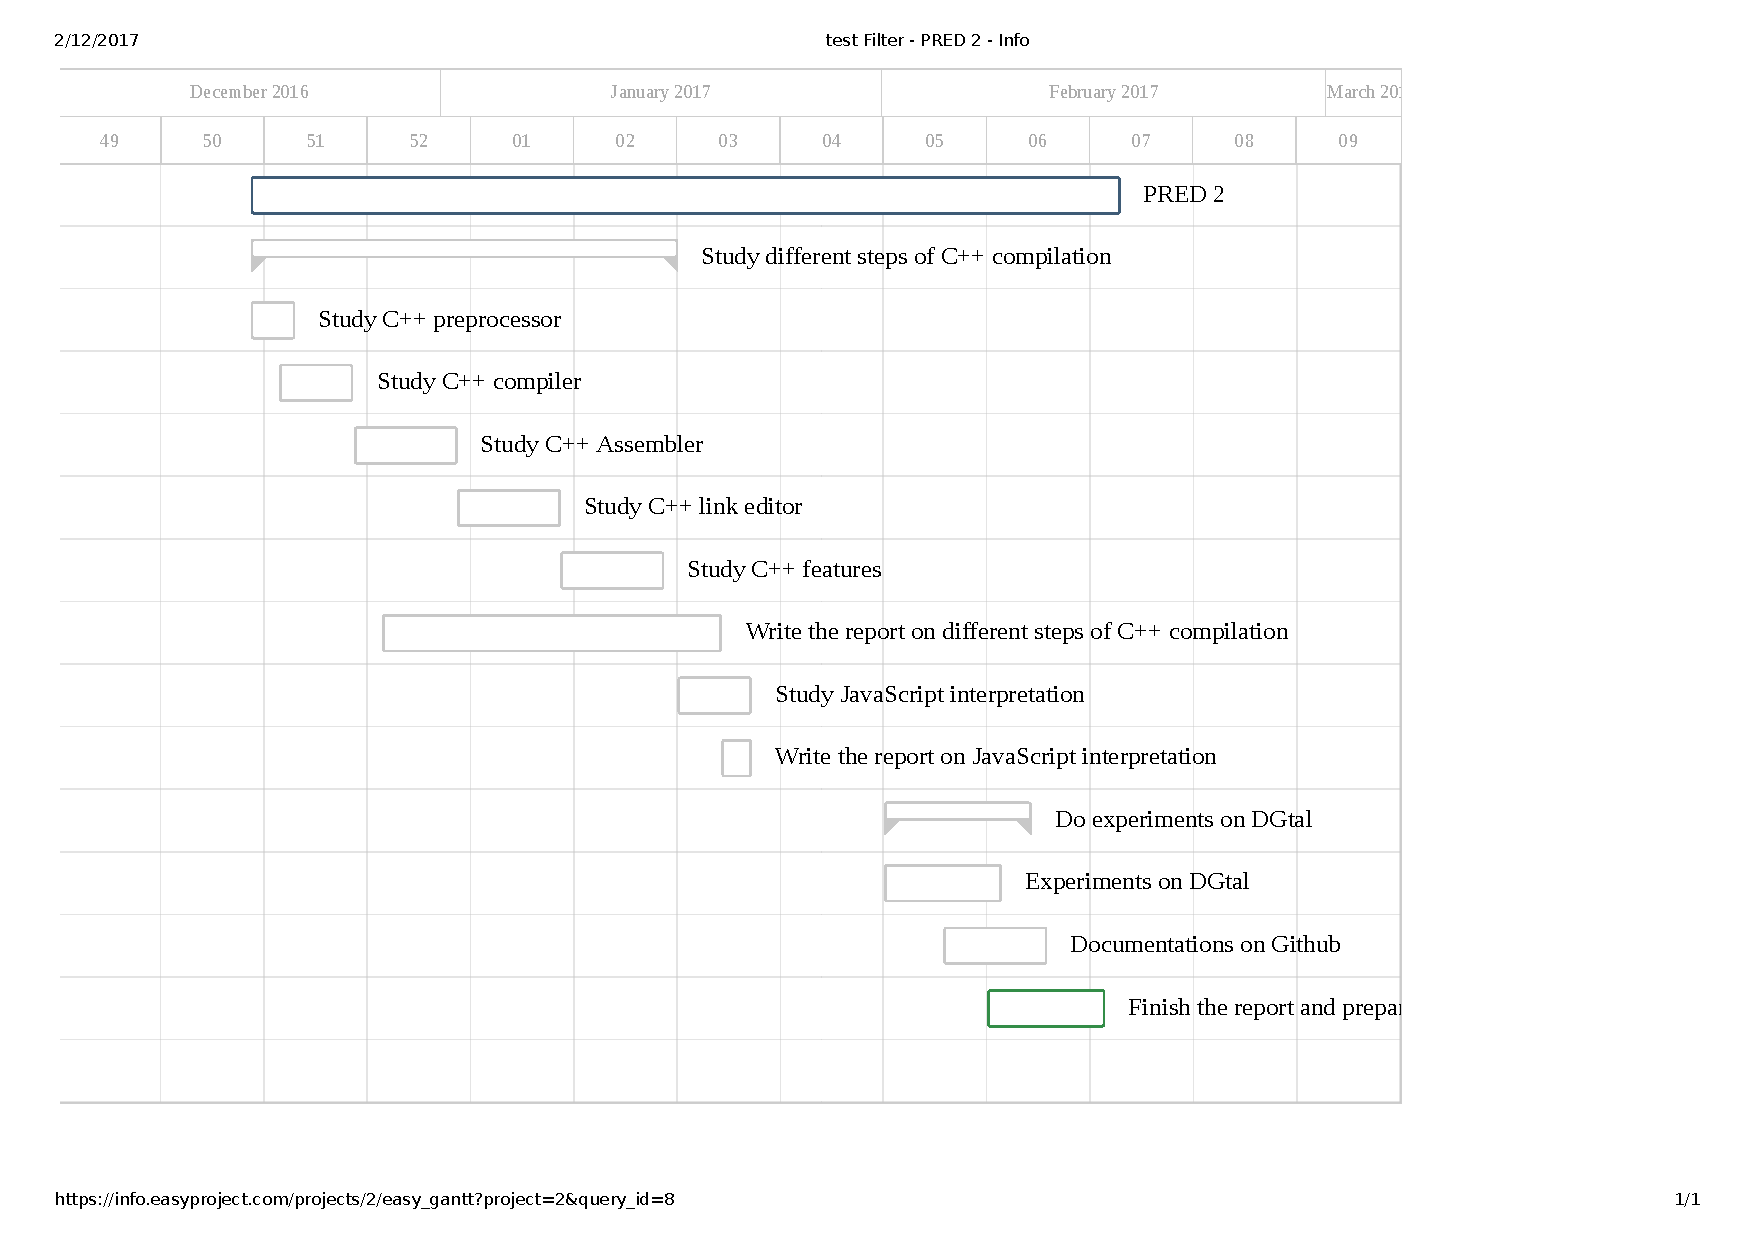
\includegraphics[scale=0.6]{Images/Gantt4.pdf}
      \caption{Planning 2}
   \label{fig:Planning2}
\end{figure*}


\begin{comment}
Discuss differences between the drafting and the planning as well as lessons learned on the management of a research project or R\&D project.
\end{comment}
